\documentclass[12pt]{beamer}
%\documentclass[20pt,handout]{beamer}
\usetheme{Darmstadt}
\usepackage{graphicx}
%\usepackage[german]{babel}
\usepackage{ngerman}
\usepackage[T1]{fontenc}
\usepackage[utf8]{inputenc}
\usepackage{tikz}
\setbeamertemplate{footline}[frame number]

\newcommand{\cc}[1]{\includegraphics[height=4mm]{img/#1.png}\hspace{1mm}}
\usepackage{ifthen}
\newcommand{\license}[2][]{\\#2\ifthenelse{\equal{#1}{}}{}{\\\scriptsize\url{#1}}}
\usepackage{textcomp}
\usepackage{hyperref}

\pgfdeclareimage[height=.6cm]{c3d2logo}{./img/c3d2.pdf} 


\pgfdeclarelayer{foreground}
\pgfsetlayers{main,foreground}
\logo{\pgfputat{\pgfxy(-1,0)}{\pgfbox[center,base]{\pgfuseimage{c3d2logo}}}}


\title{NSA, Prism und co - Wie schützt man sich vor Überwachung?}
\author{\small Marius Melzer\\\large Chaos Computer Club Dresden}
\date{26.11.2013}

\begin{document}
\maketitle

\section{Einleitung}
\subsection{}

\begin{frame}
  \frametitle{Chaos Computer Club}
  \begin{figure}
    
\includegraphics[height=0.7\textheight]{img/fingerabdruck.jpg}
  \end{figure}
\end{frame}

\begin{frame}
  \frametitle{Chaos Computer Club}
  \begin{figure}
    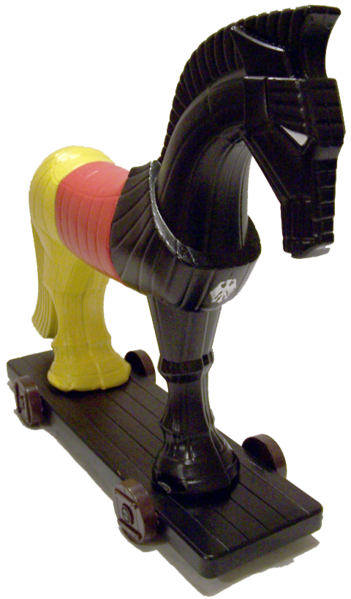
\includegraphics[height=0.7\textheight]{img/trojaner.png}
  \end{figure}
\end{frame}

\begin{frame}
    \frametitle{Chaos Computer Club}
    \begin{itemize}
      \item<1-> Chaos Computer Club Dresden (\url{http://c3d2.de})
          \note{}
      \item<2-> Datenspuren: Herbst 2014 \url{http://datenspuren.de}
      \item<3-> Podcasts (\url{http://pentamedia.de})
      \item<4-> Chaos macht Schule
    \end{itemize}
\end{frame}

\begin{frame}
    \frametitle{Bundespräsident Gauck zur NSA-Überwachung}
    \begin{center}
      "`Wir wissen z.B., dass es nicht so ist, wie bei der Stasi und dem KGB, dass es dicke Aktenbände gibt, wo unsere Gesprächsinhalte alle aufgeschrieben und schön abgeheftet sind. Das ist es nicht."'
      \end{center}
\end{frame}

\begin{frame}
    \frametitle{Stasi vs. NSA}
    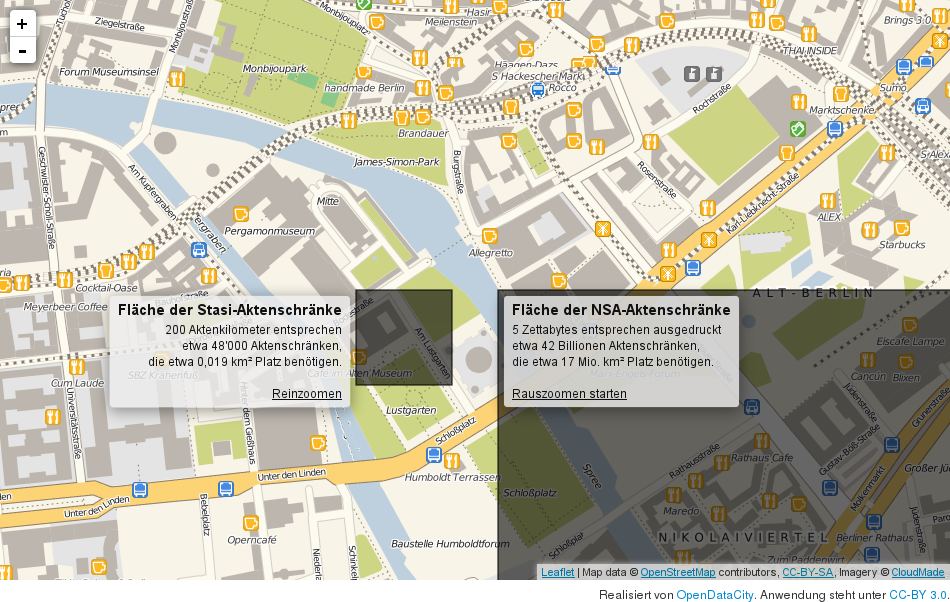
\includegraphics[height=0.7\textheight]{img/akten1.png}
\end{frame}

\begin{frame}
    \frametitle{Stasi vs. NSA}
    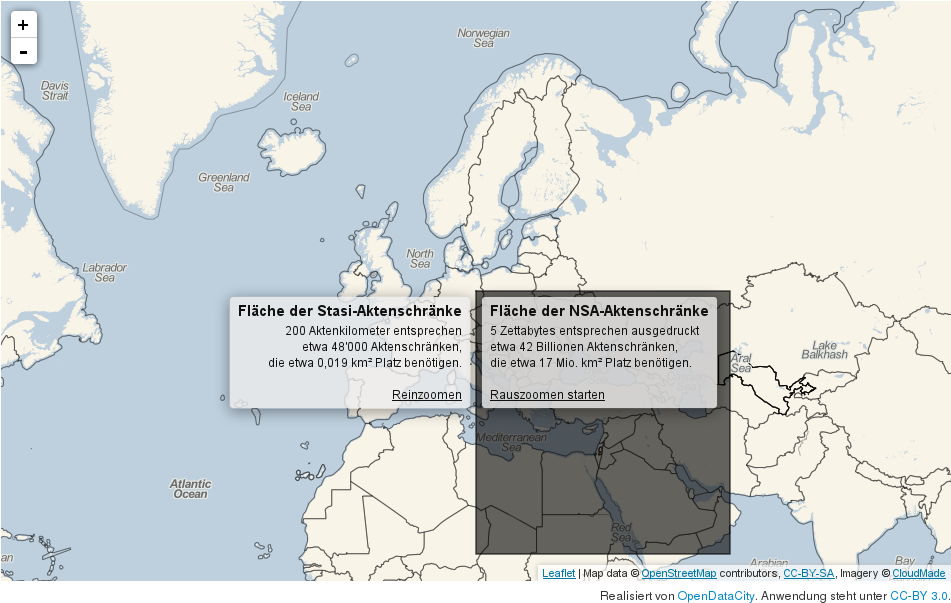
\includegraphics[height=0.7\textheight]{img/akten2.png}
\end{frame}

\begin{frame}
    \frametitle{Merkels Handy}
    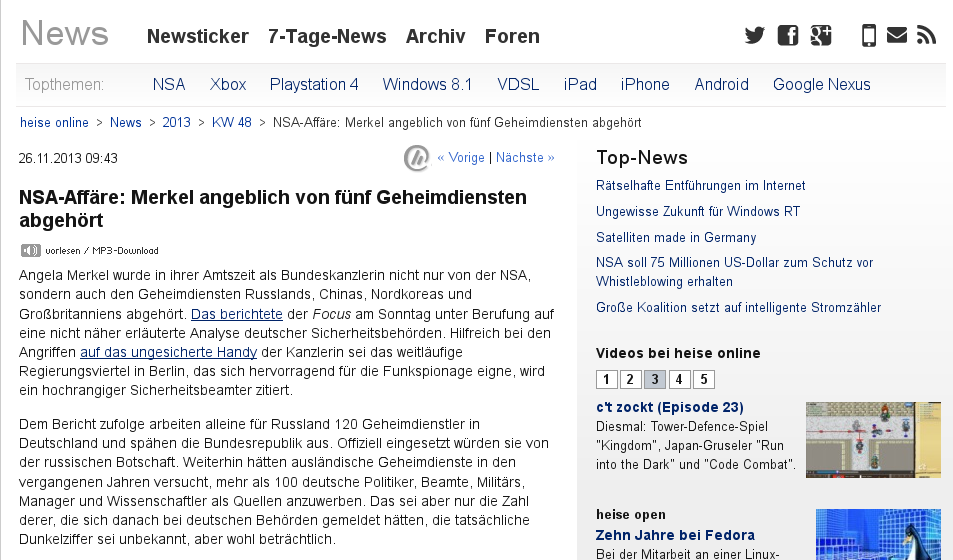
\includegraphics[height=0.7\textheight]{img/heise-merkel.png}
\end{frame}

\begin{frame}
    \frametitle{Wem nützen meine Daten?}
    \begin{itemize}
      \item<2-> Unternehmen
        \begin{itemize}
          \item<3-> (Zielgerichtete) Werbung
          \item<4-> Tracking
        \end{itemize}
      \item<5-> Staat, Geheimdienste
        \begin{itemize}
          \item<6-> Terrorismusbekämpfung? Kinderpornographie?
          \item<7-> Macht
        \end{itemize}
      \item<8->Meine Mitmenschen
        \begin{itemize}
          \item<9-> ?
      \end{itemize}
    \end{itemize}
\end{frame}

\begin{frame}
    \frametitle{Wie schütze ich mich?}
    \begin{itemize}
      \item<1-> technisch
      \item<2-> Verhalten
    \end{itemize}
\end{frame}

\begin{frame}
    \frametitle{Wie kommunizieren wir im Internet?}
    \begin{center}
      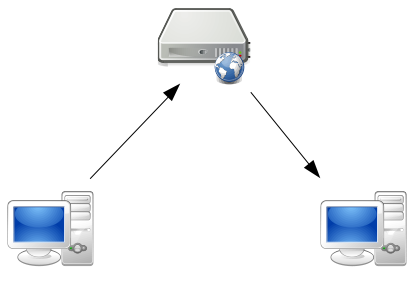
\includegraphics[height=5cm]{img/c-s.png}
    \end{center}
\end{frame}

\begin{frame}
    \frametitle{Föderation}
    \begin{center}
      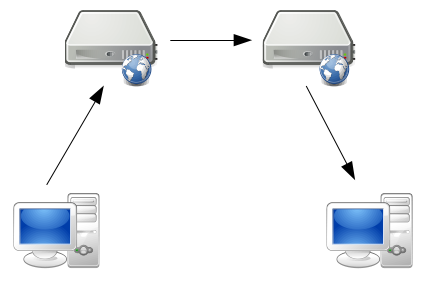
\includegraphics[height=5cm]{img/fed.png}
    \end{center}
\end{frame}

\begin{frame}
    \frametitle{P2P}
    \begin{center}
      
\includegraphics[width=7cm]{img/direkt.png}
    \end{center}
\end{frame}

\begin{frame}
    \frametitle{P2P: Praxis-Beispiel: https://palava.tv}
    \begin{center}
      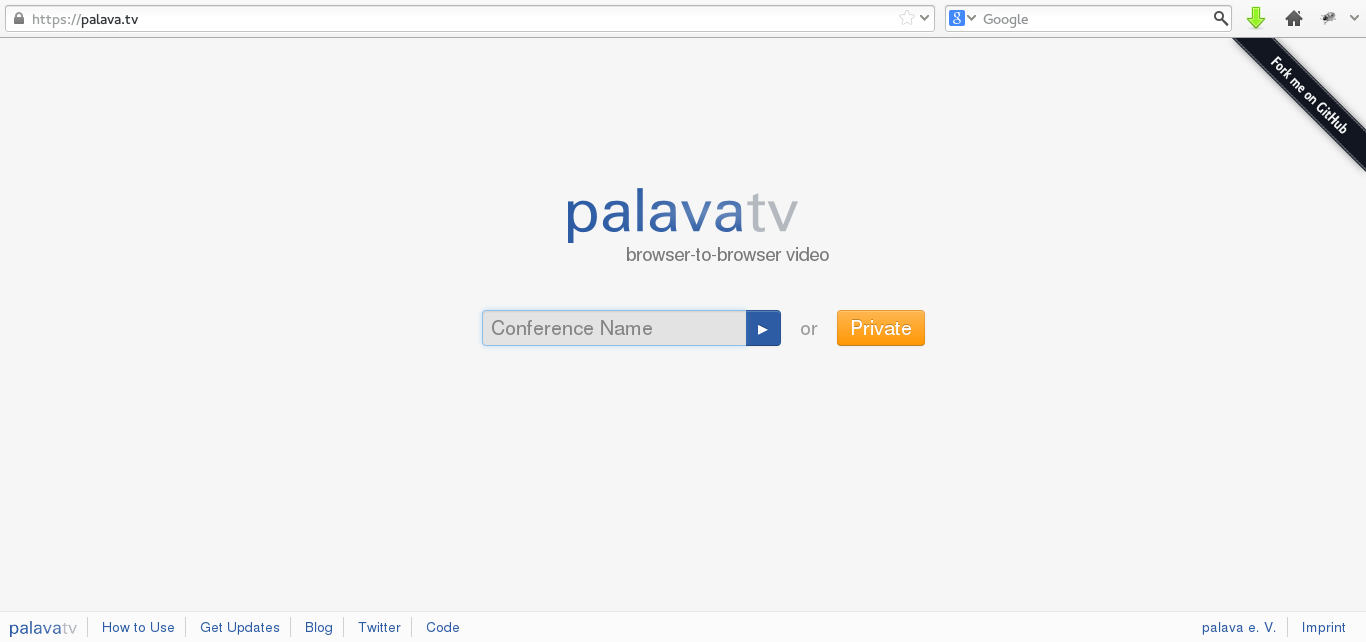
\includegraphics[width=\linewidth]{img/palava.png}
    \end{center}
\end{frame}

\begin{frame}
    \frametitle{Was ist zu schützen?}
    \begin{center}
      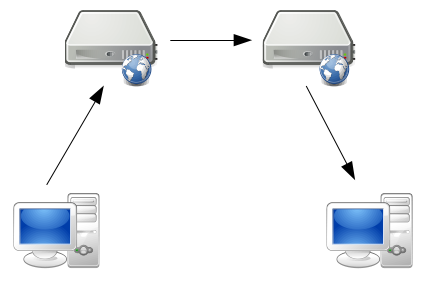
\includegraphics[height=5cm]{img/fed.png}
    \end{center}
\end{frame}

\section{Angriff von außen}
\subsection{}

\begin{frame}
    \frametitle{Was ist zu schützen?}
    \begin{center}
      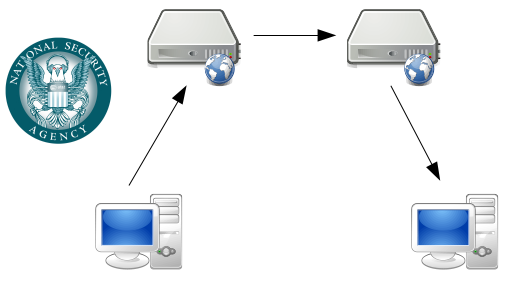
\includegraphics[height=5cm]{img/fed-bad-guy.png}
    \end{center}
\end{frame}

\begin{frame}
    \frametitle{Was ist zu schützen?}
    \begin{center}
      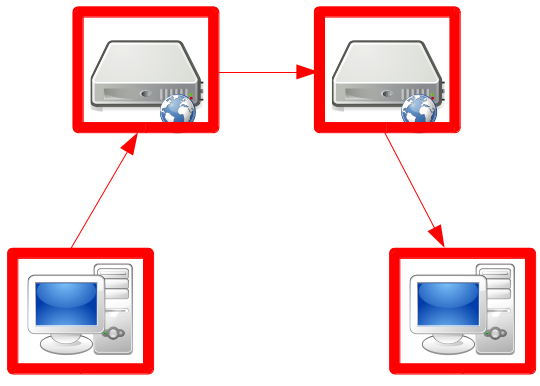
\includegraphics[height=5cm]{img/fed-none.png}
    \end{center}
\end{frame}

\begin{frame}
    \frametitle{Wie schütze ich meinen Computer?}
    \begin{itemize}
      \item Virenscanner
      \item Firewall
      \item Aktuelle und vertrauenswürdige Software
    \end{itemize}
\end{frame}

\begin{frame}
    \frametitle{Wie schütze ich mein Smartphone?}
    \begin{itemize}
      \item Permissions
      \item Firewall (z.B. AFwall+: https://f-droid.org/repository/browse/?fdid=dev.ukanth.ufirewall)
      \item Aktuelle und vertrauenswürdige Software
    \end{itemize}
\end{frame}

\begin{frame}
    \frametitle{Vertrauenswürdige Software?}
    \begin{center}\Large
        Einer Software, die nicht quelloffen ist, kann man nicht vertrauen
    \end{center}
\end{frame}

\begin{frame}
    \frametitle{Open Source Software}
    \begin{center}
      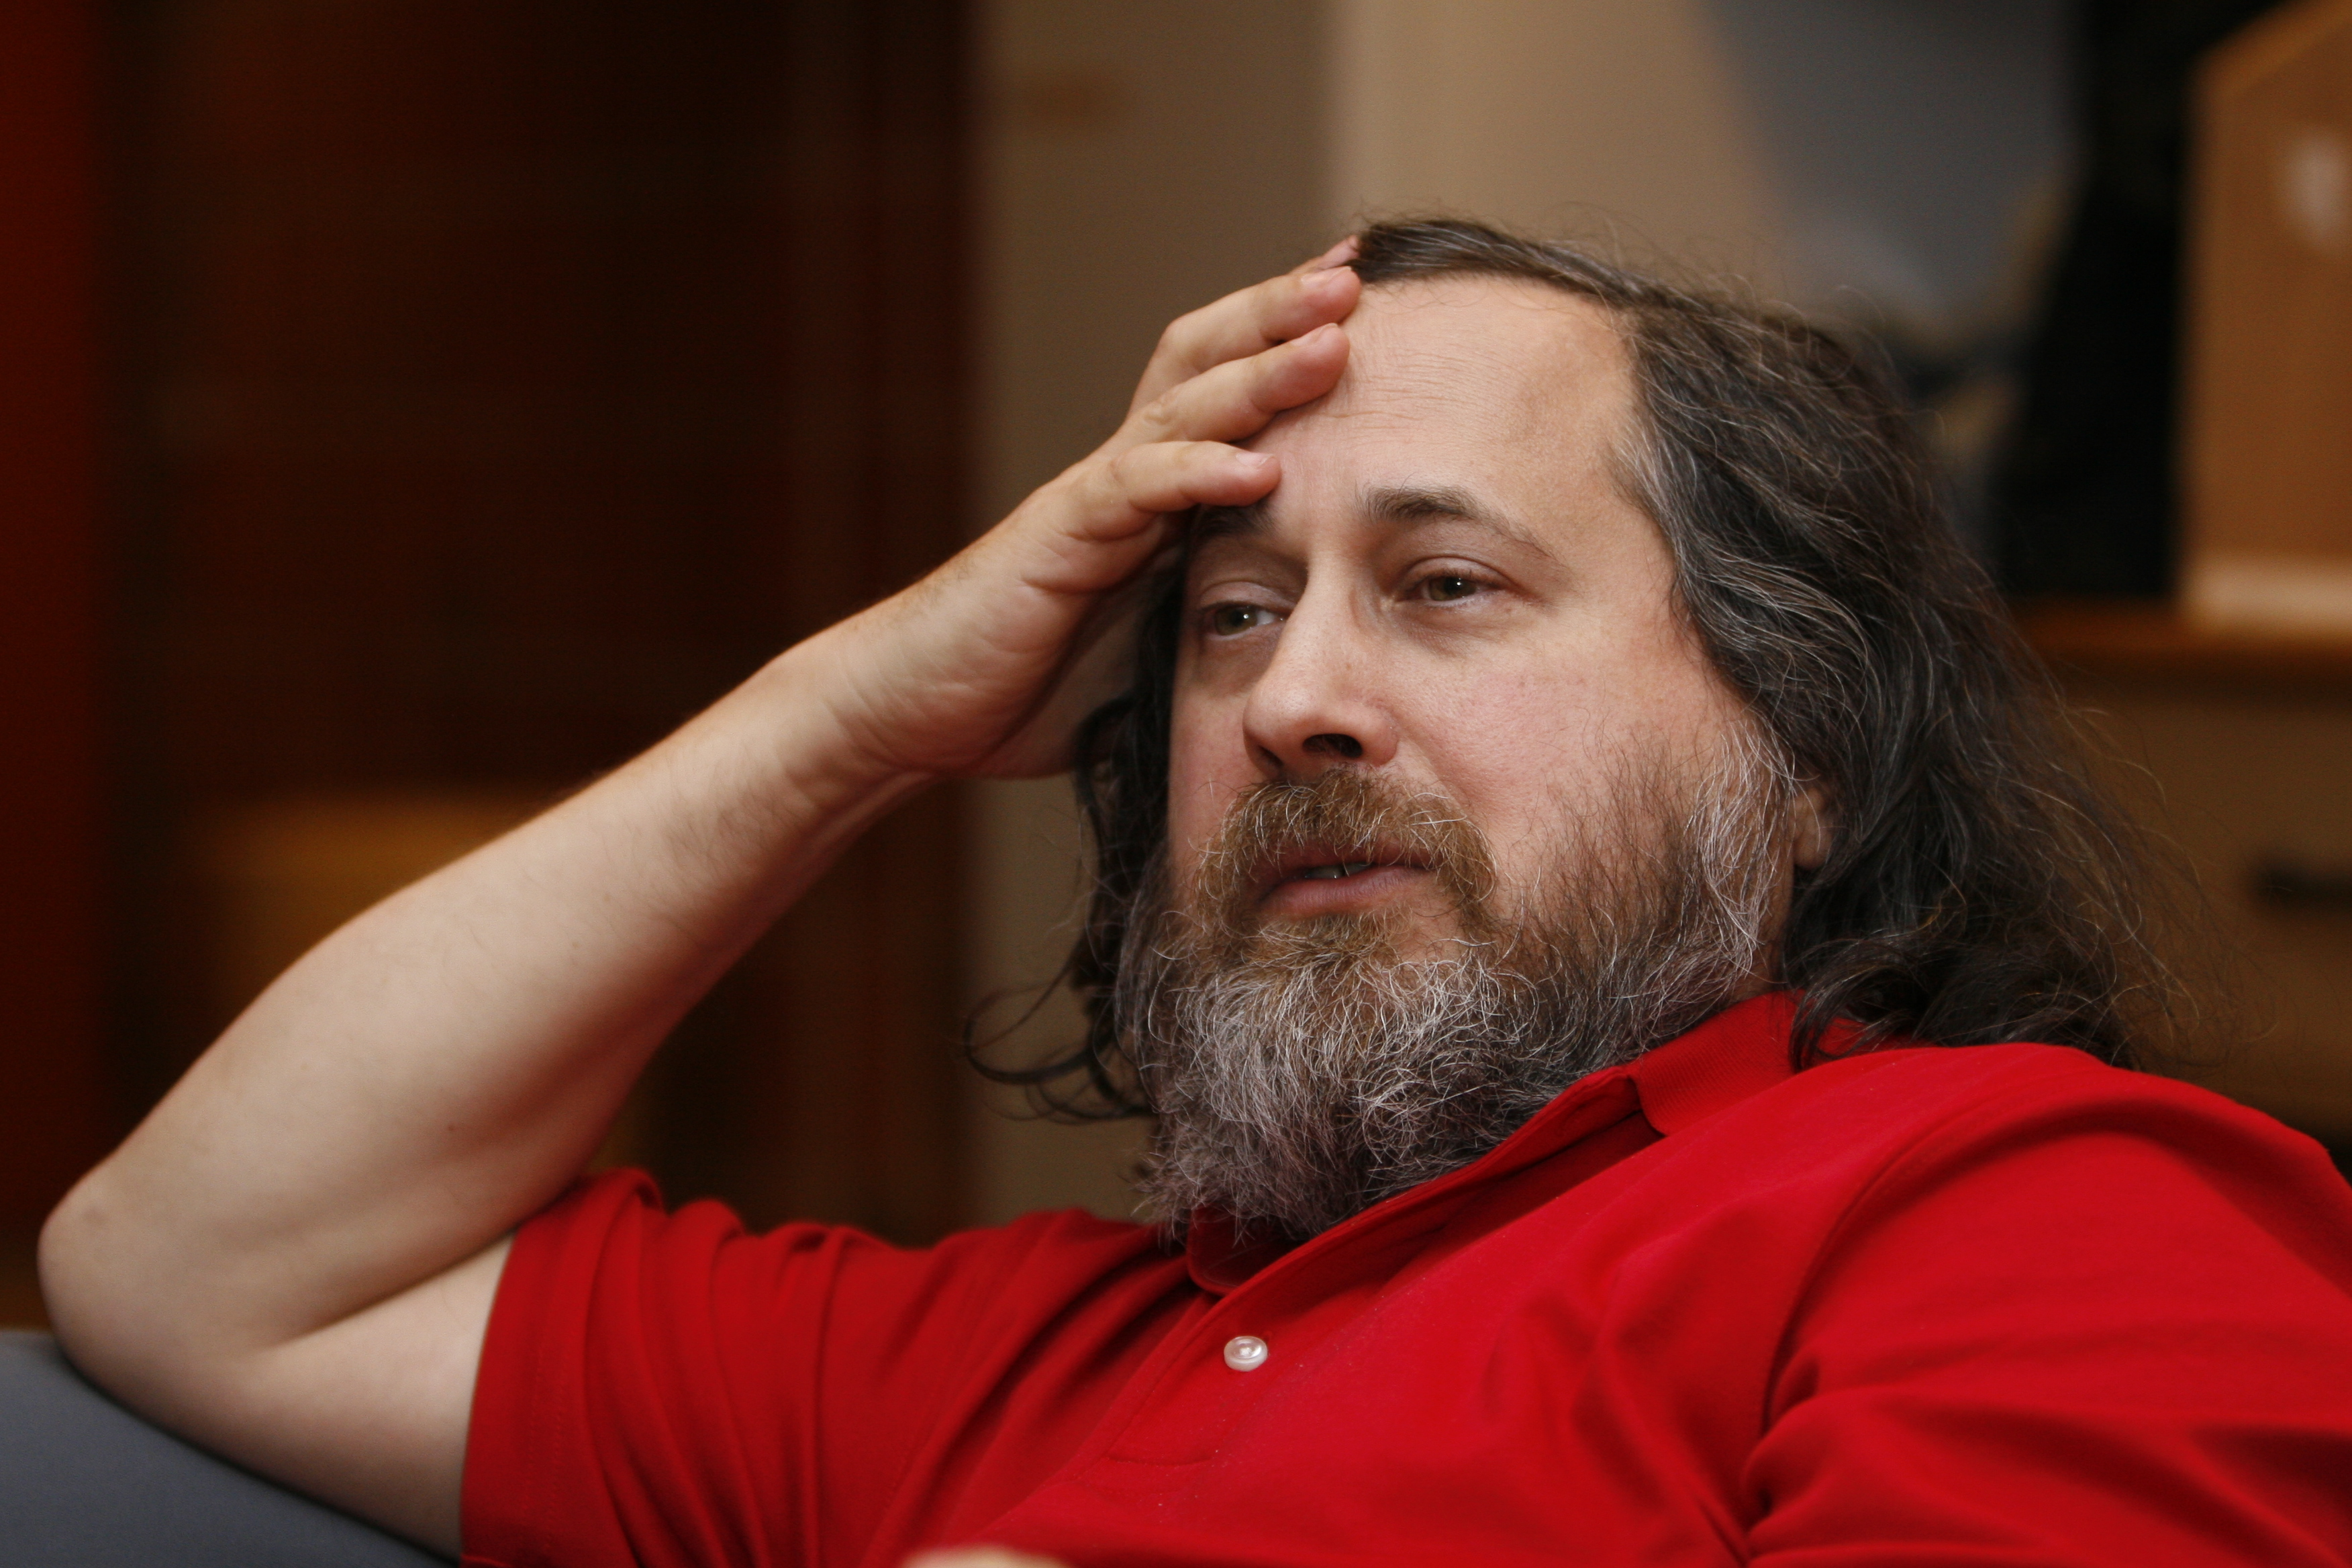
\includegraphics[height=0.7\textheight]{img/stallman.jpg}
      \\{\small \cc{by} Anders Brenna}
    \end{center}
\end{frame}

\begin{frame}
    \frametitle{Open Source Software für den PC}
    \begin{itemize}
      \item Firefox
      \item Thunderbird
      \item Libreoffice
      \item Gimp
      \item Blender
    \end{itemize}
\end{frame}

\begin{frame}
    \frametitle{Open Source Betriebssysteme für den PC}
    \begin{itemize}
      \item Linux-Distributionen (Ubuntu, Linux Mint)
        \begin{itemize}
          \item Wine
      \end{itemize}
      \item BSD
    \end{itemize}
\end{frame}

\begin{frame}
    \frametitle{Linux mit Gnome}
    \begin{center}
      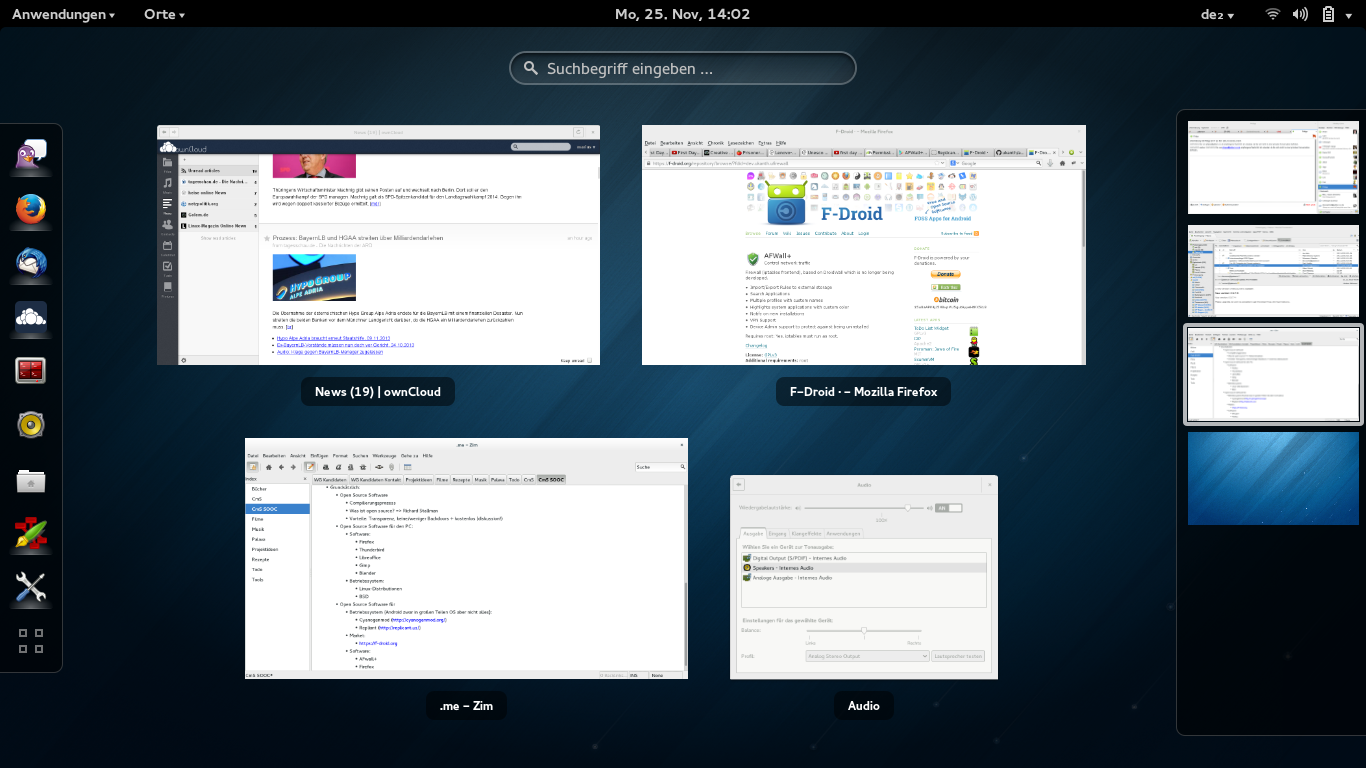
\includegraphics[height=0.7\textheight]{img/gnome.png}
    \end{center}
\end{frame}

\begin{frame}
    \frametitle{Open Source Betriebssysteme fürs Handy}
    \begin{itemize}
      \item Cyanogenmod (http://cyanogenmod.org/)
      \item Replicant (http://replicant.us/)
      \item Firefox OS (http://www.mozilla.org/de/firefox/os/) - hat Web Apps
      \item Sailfish OS (https://sailfishos.org/) - kann Android Apps
    \end{itemize}
\end{frame}

\begin{frame}
    \frametitle{Open Source Software fürs Smartphone}
    \begin{itemize}
      \item Market: F-Droid (https://f-droid.org)
      \item Firefox
      \item ...
    \end{itemize}
\end{frame}

\begin{frame}
    \frametitle{Zusammenfassung}
    \begin{itemize}
      \item Computer/Handy absichern
      \item Open Source Software verwenden
    \end{itemize}
\end{frame}

\begin{frame}
    \frametitle{Was ist zu schützen?}
    \begin{center}
      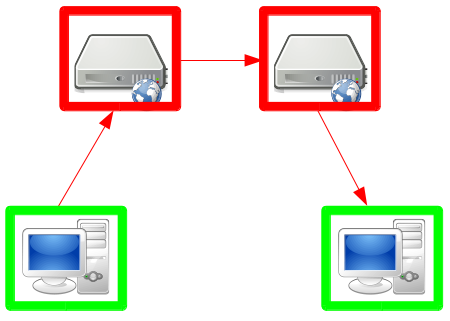
\includegraphics[height=5cm]{img/fed-clients.png}
    \end{center}
\end{frame}

\begin{frame}
    \frametitle{Schützen der Verbindung}
    \begin{itemize}
      \item Vertraulichkeit
      \item Integrität
      \item Anonymität
    \end{itemize}
\end{frame}

\begin{frame}
    \frametitle{Verschlüsselung}
    \begin{itemize}
      \item<2-> symetrische Verschlüsselung
      \item<3-> asymetrische Verschlüsselung
      \item<4-> Woher kommt Vertrauen?
    \end{itemize}
\end{frame}

\begin{frame}
    \frametitle{SSL / TLS}
    \begin{itemize}
      \item<2-> eingesetzt im Web, Mail, ...
      \item<3-> hierarchische Struktur
      \item<4-> gespeicherte Liste von vertrauenswürdigen Zertifikaten
    \end{itemize}
\end{frame}

\begin{frame}
    \frametitle{Von Firefox vertraute Zertifikate}
    \begin{center}
      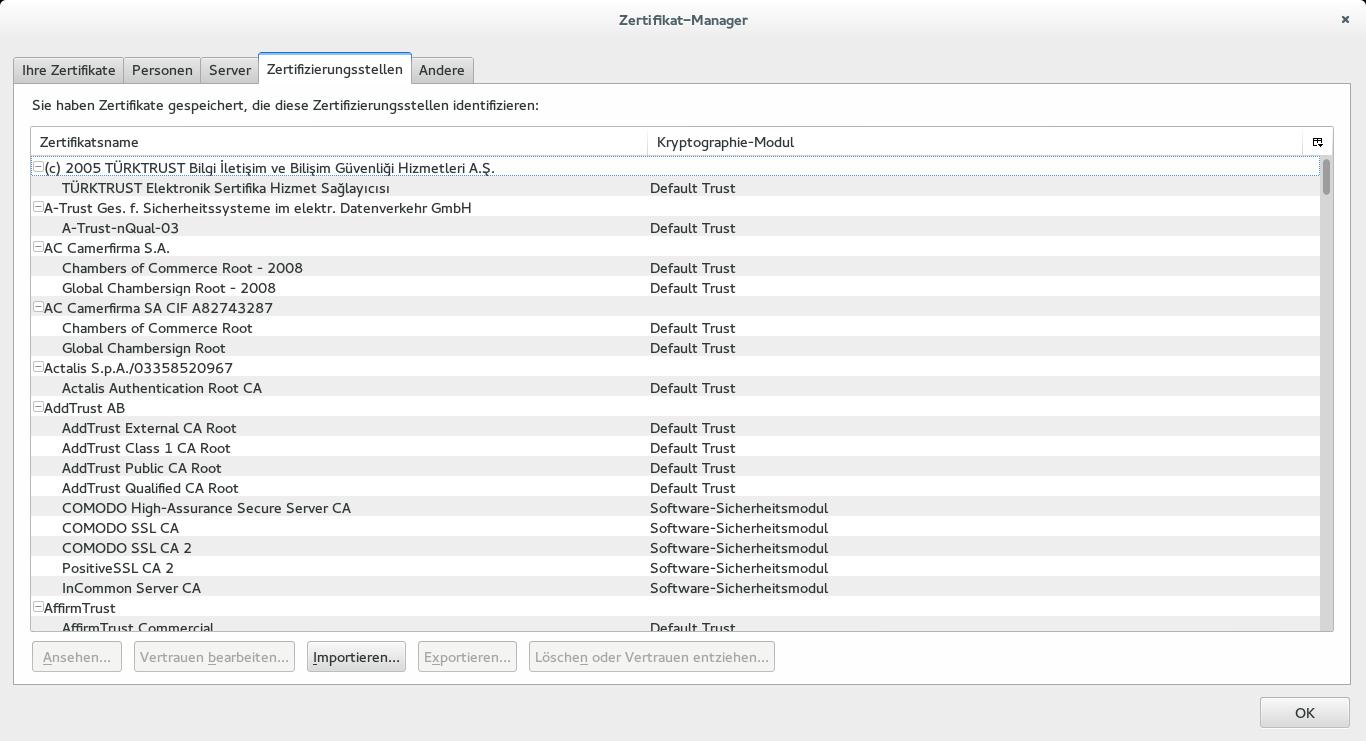
\includegraphics[height=5cm]{img/zertifikate.png}
    \end{center}
\end{frame}

\begin{frame}
    \frametitle{Anonymität}
    \begin{center}
      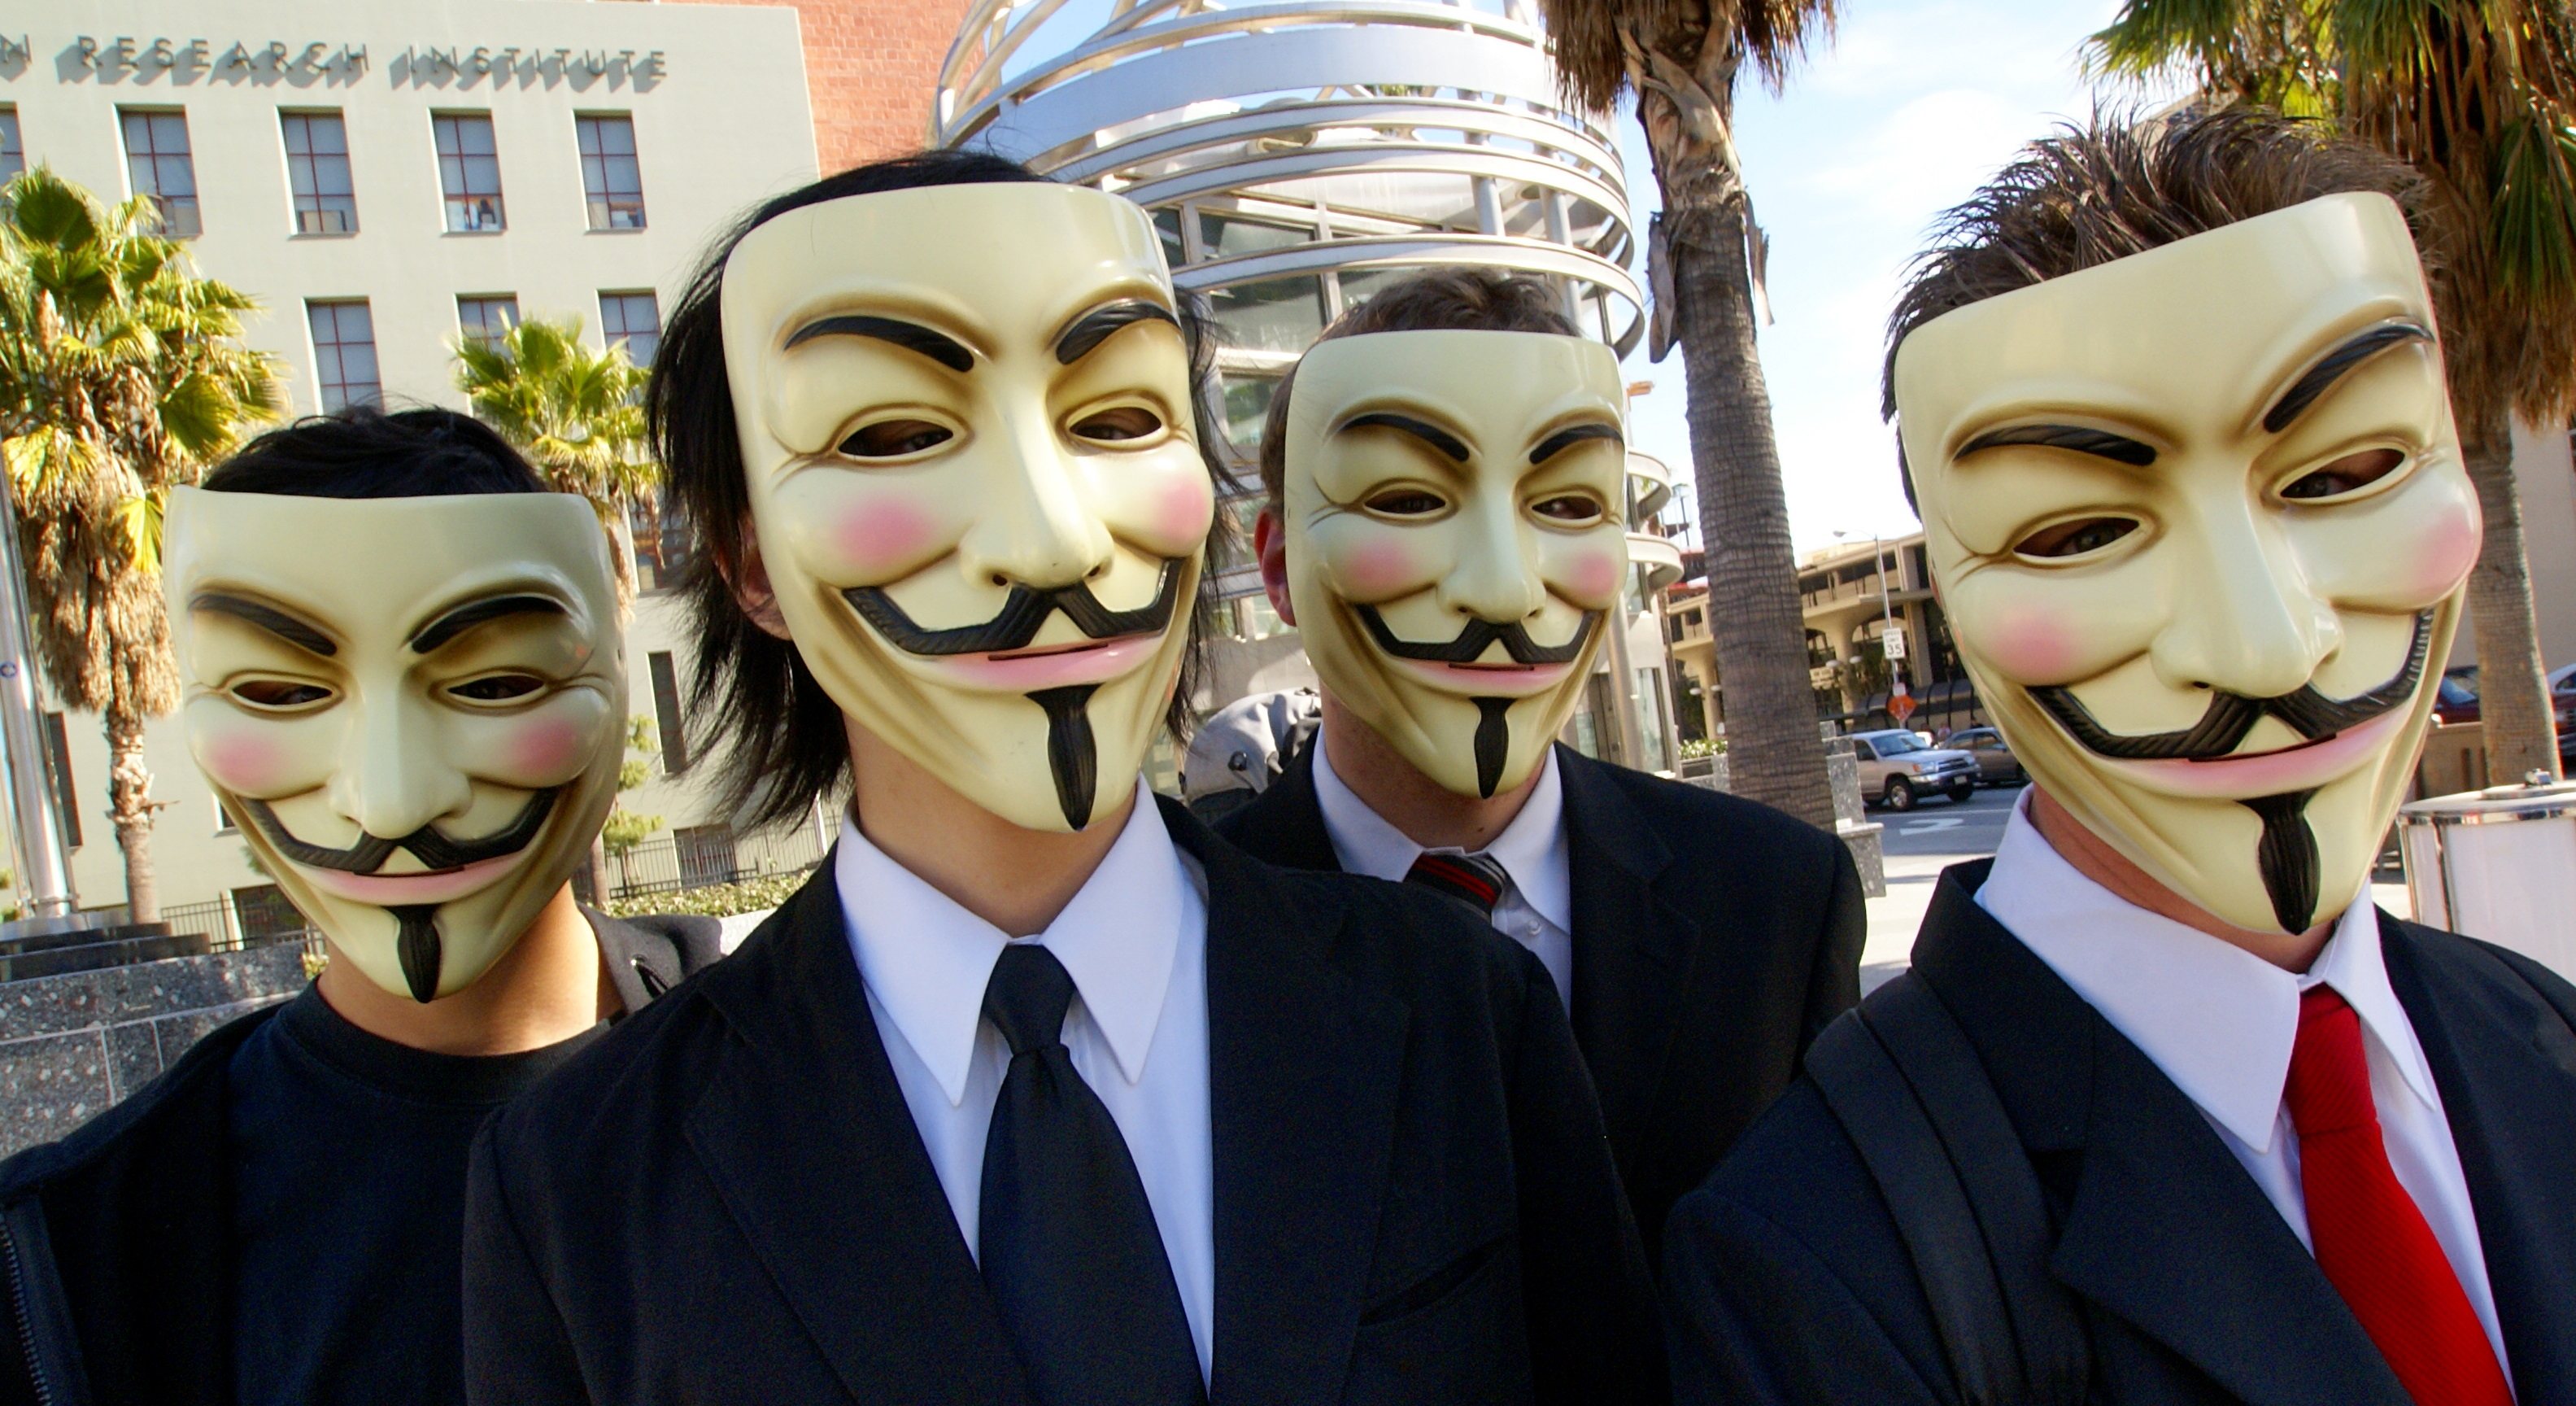
\includegraphics[height=5cm]{img/anonymous.jpg}
      \\{\small \cc{by-sa} Vincent Diamante}
    \end{center}
\end{frame}

\begin{frame}
    \frametitle{Metadaten}
    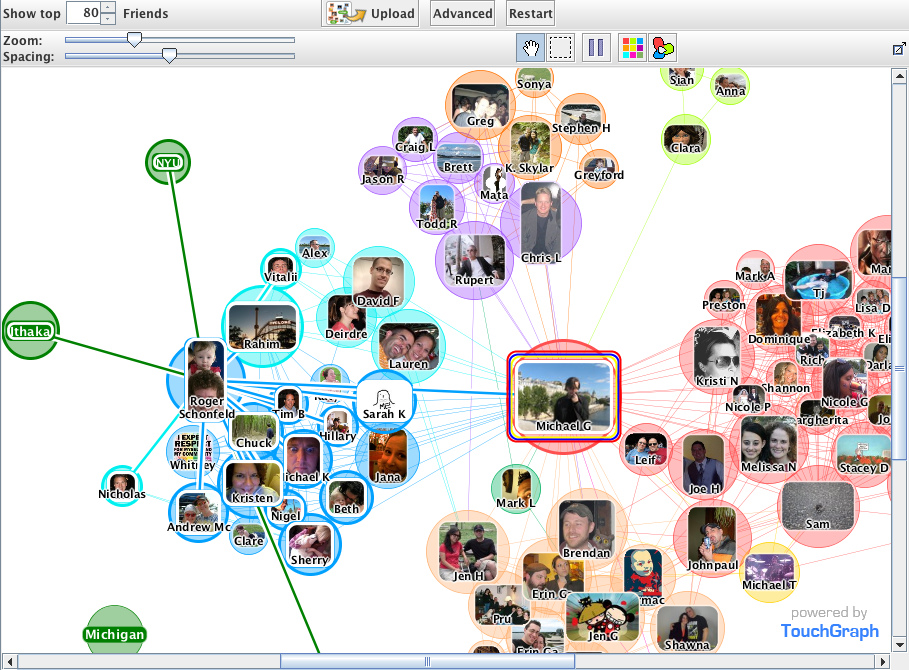
\includegraphics[height=0.7\textheight]{img/socialgraph.jpg}
    \\{\small \cc{by-sa} Michael Sean Gallagher}
\end{frame}

\begin{frame}
    \frametitle{Metadaten}
    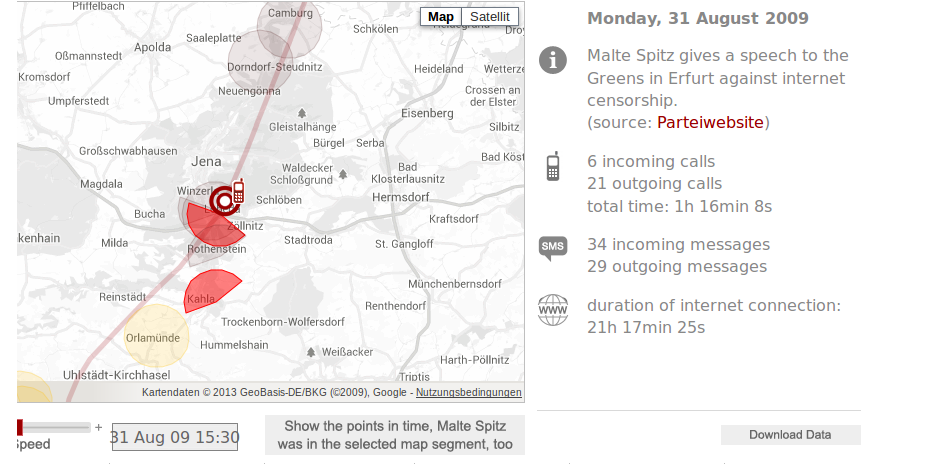
\includegraphics[height=0.7\textheight]{img/maltespitz.png}
\end{frame}

\begin{frame}
    \frametitle{TOR}
    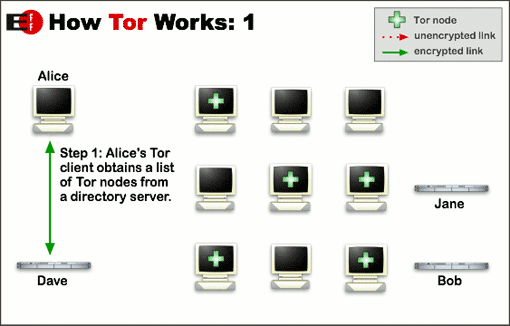
\includegraphics[height=0.7\textheight]{img/tor1.png}
    \\{\small \cc{by} The Tor Project}
\end{frame}

\begin{frame}
    \frametitle{TOR}
    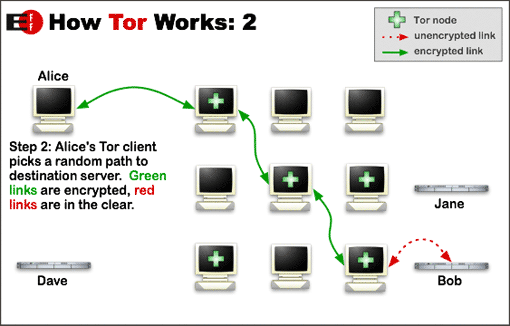
\includegraphics[height=0.7\textheight]{img/tor2.png}
    \\{\small \cc{by} The Tor Project}
\end{frame}

\begin{frame}
    \frametitle{TOR}
    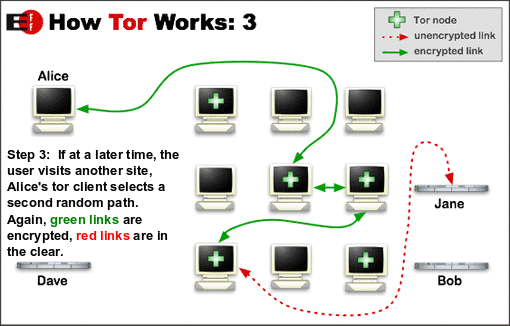
\includegraphics[height=0.7\textheight]{img/tor3.png}
    \\{\small \cc{by} The Tor Project}
\end{frame}

\begin{frame}
    \frametitle{TOR}
    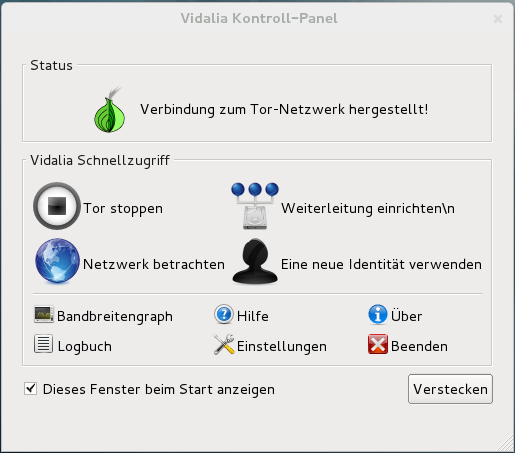
\includegraphics[height=0.7\textheight]{img/vidalia.png}
\end{frame}

\begin{frame}
    \frametitle{TOR}
    \begin{center} \Large Bridges \end{center}
\end{frame}

\begin{frame}
    \frametitle{TOR}
    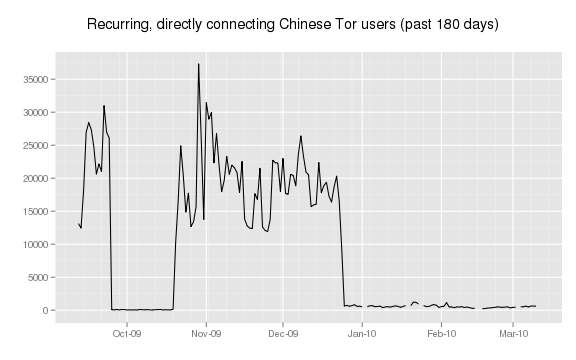
\includegraphics[height=0.7\textheight]{img/bridge1.png}
\end{frame}

\begin{frame}
    \frametitle{TOR}
    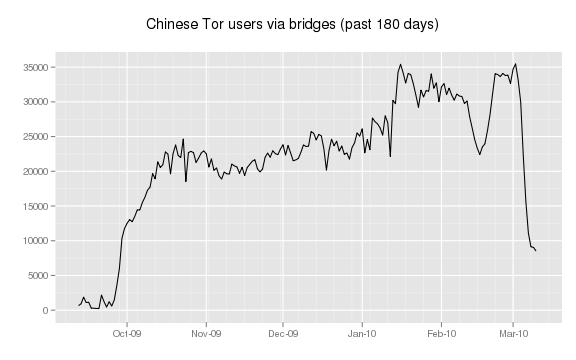
\includegraphics[height=0.7\textheight]{img/bridge2.png}
\end{frame}

\begin{frame}
    \frametitle{Anonymität unter Vollüberwachung}
    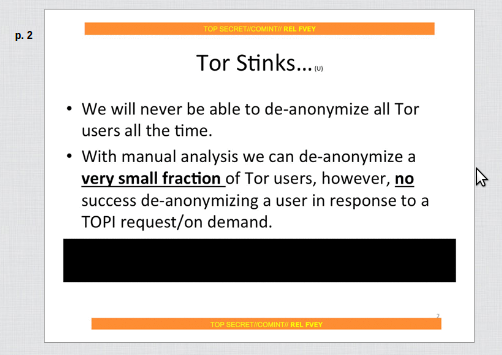
\includegraphics[height=0.7\textheight]{img/torstinks.png}
\end{frame}

\begin{frame}
    \frametitle{Zensur}
    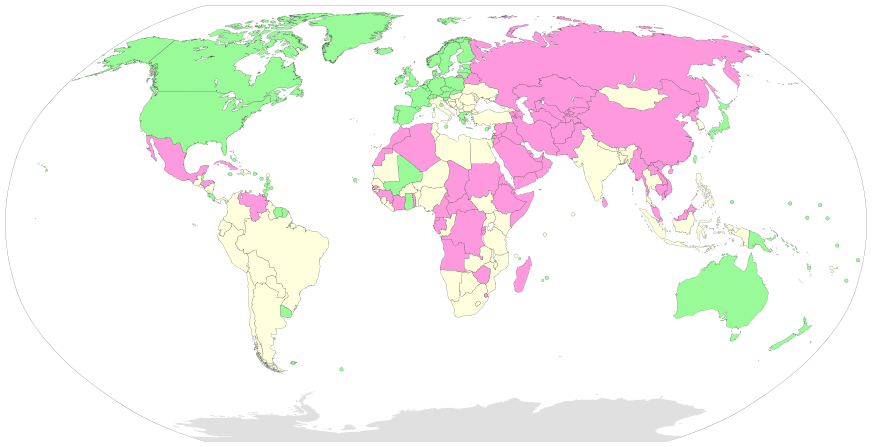
\includegraphics[height=0.7\textheight]{img/zensur.png}
    \\{\small \cc{by-sa} Jeff Ogden (W163)}
\end{frame}

\begin{frame}
    \frametitle{Was ist zu schützen?}
    \begin{center}
      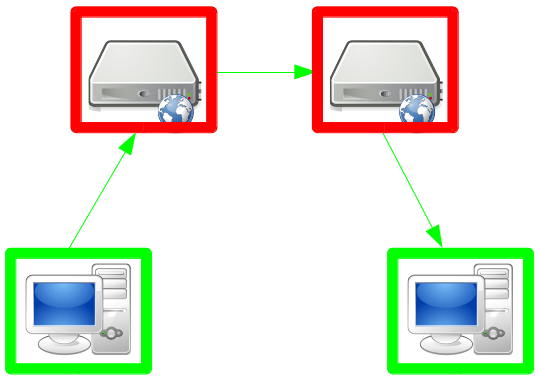
\includegraphics[height=5cm]{img/fed-clients-comm.png}
    \end{center}
\end{frame}

\begin{frame}
    \frametitle{Was ist zu schützen?}
    \begin{center}
      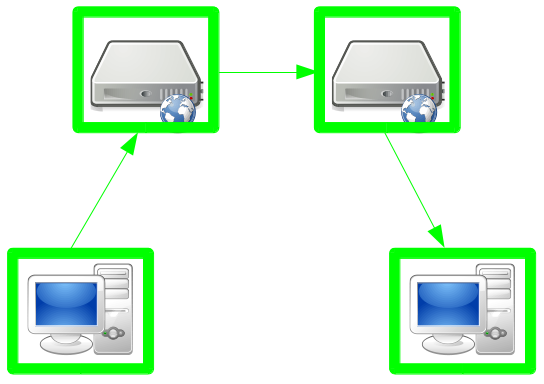
\includegraphics[height=5cm]{img/fed-all.png}
    \end{center}
\end{frame}

\section{Angriff von innen}
\subsection{}

\begin{frame}
    \frametitle{Was ist zu schützen?}
    \begin{center}
      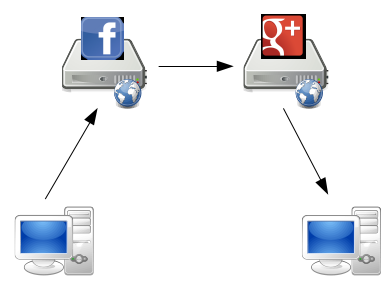
\includegraphics[height=5cm]{img/fed-social.png}
    \end{center}
\end{frame}

\begin{frame}
    \frametitle{Metadaten - Lightbeam}
    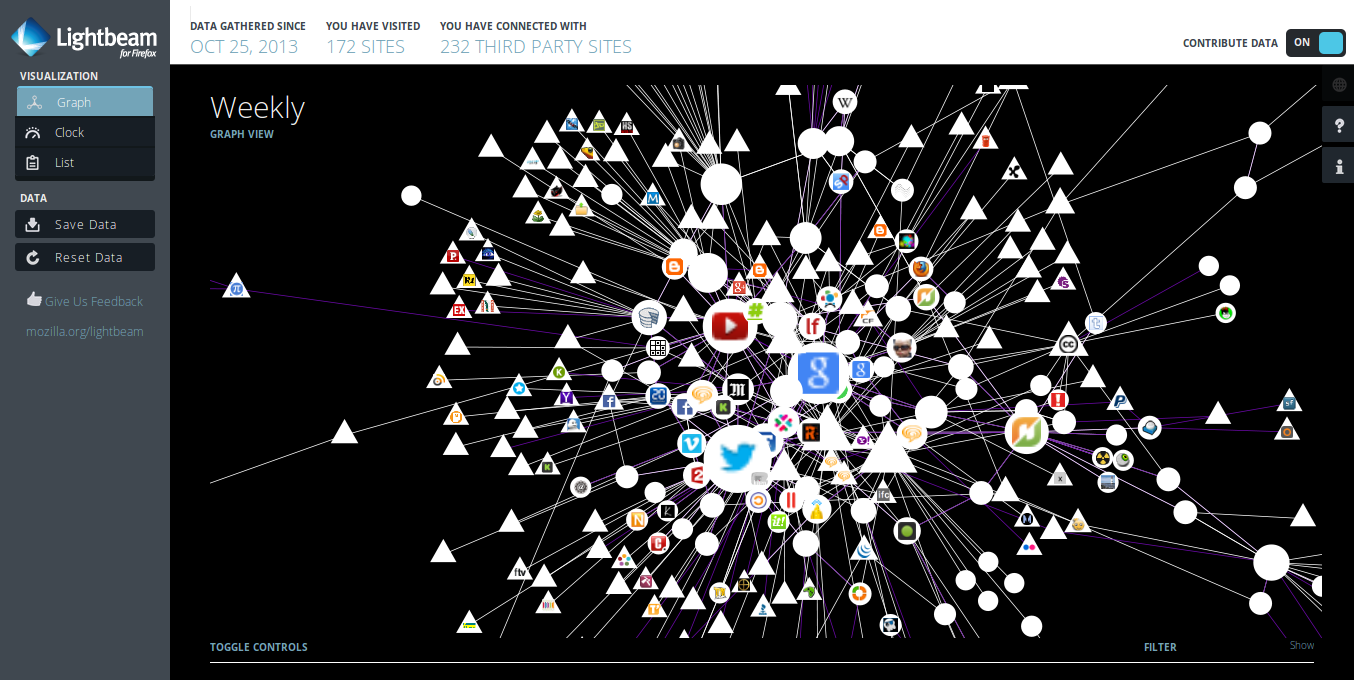
\includegraphics[height=0.7\textheight]{img/lightbeam.png}
    \\{\small \cc{by-sa} Clint Lalonde}
\end{frame}

\begin{frame}
    \frametitle{Unterscheidung}
    \begin{itemize}
      \item<2-> Ich will etwas vom Server
        \begin{itemize}
          \item<3-> Cookies
          \item<4-> => Third-Party-Cookies ausschalten
          \item<5-> => Cookies nach Session löschen
          \item<6-> Zähl-/Tracking-Pixel, ...
          \item<7-> => Ghostery
          \item<8-> => TOR
        \end{itemize}
    \end{itemize}
\end{frame}

\begin{frame}
    \frametitle{Unterscheidung}
    \begin{itemize}
      \item<2-> Ich will etwas vom Server
        \begin{itemize}
          \item<3-> Pseudonymität
          \item<4-> Daten ausdenken
          \item<5-> Mailinator
        \end{itemize}
    \end{itemize}
\end{frame}

\begin{frame}
    \frametitle{Unterscheidung}
    \begin{itemize}
      \item<2-> Ich will etwas von einem anderen Nutzer
      \item<3-> => Ende-zu-Ende-Verschlüsselung
    \end{itemize}
\end{frame}

\begin{frame}
    \frametitle{Ende-zu-Ende-Verschlüsselung}
    \begin{center}
      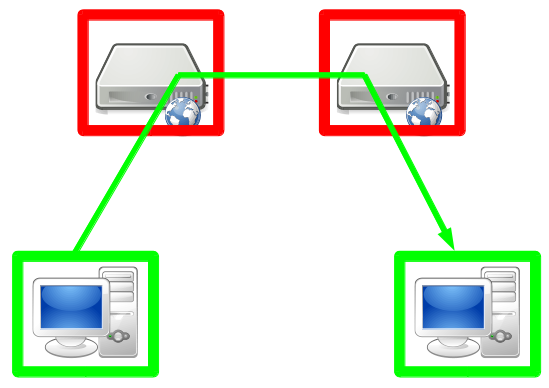
\includegraphics[height=5cm]{img/fed-end-to-end.png}
    \end{center}
\end{frame}

\begin{frame}
    \frametitle{Web of Trust}
    \begin{center}
      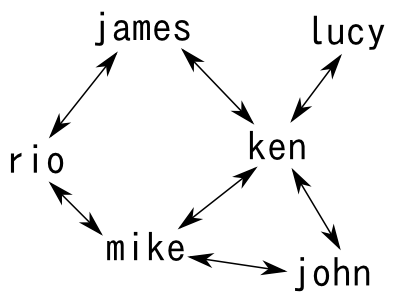
\includegraphics[height=5cm]{img/weboftrust.png}
      \\{\small \cc{by-sa} Koichi Akabe}
    \end{center}
\end{frame}

\begin{frame}
    \frametitle{Ende-zu-Ende-Verschlüsselung in der Praxis}
    \begin{itemize}
      \item<2-> GPG für Email (Plugin für Thunderbird: https://addons.mozilla.org/de/thunderbird/addon/enigmail/)
      \item<3-> OTR für Jabber:
        \begin{itemize}
          \item Pidgin mit OTR-Plugin für Linux und Windows
          \item GibberBot oder Xabber für Android
          \item Adium für Mac, ChatSecure für iOS
        \end{itemize}
      \item<4-> palava.tv für Videotelefonie
      \item<5-> Redphone für Handytelefonate (Android)
      \item<6-> TextSecure für SMS (Android)
    \end{itemize}
\end{frame}

\section{Ende}
\subsection{}

\begin{frame}
  \frametitle{Diskussion}
  \begin{center}
    {\Large Diskussion}\\
    \vspace{5mm} 
    \href{https://github.com/c3d2/cms-nsa}{Folien}: \href{https://creativecommons.org/licenses/by-sa/4.0/}{\cc{by-sa}} Marius Melzer \\
    \vspace{4mm}
    Twitter: @faraoso, Email und Jabber: marius@rasumi.net\\GPG-Fingerprint: 52DEFC3E\\
    \vspace{4mm}
    CMS Dresden: schule@c3d2.de
  \end{center}
\end{frame}

\end{document}
